%\documentclass{sigplanconf}

% The following \documentclass options may be useful:
%
% 10pt          To set in 10-point type instead of 9-point.
% 11pt          To set in 11-point type instead of 9-point.
% authoryear    To obtain author/year citation style instead of numeric.

%\usepackage[none]{hyphenat}
%\usepackage{amsmath}
%\usepackage{mathtools}
%\usepackage{url}
%\usepackage{graphicx}
%\usepackage{placeins}
%\usepackage{fancyvrb}

%\begin{document}
%\conferenceinfo{FHPC'12,} {September 15, 2012, Copenhagen, Denmark.}
%\CopyrightYear{2012}
%\copyrightdata{978-1-4503-1577-7/12/09}

%\titlebanner{}        % These are ignored unless
%\preprintfooter{}   % 'preprint' option specified.

% \title{}
%\title{Parallel Programming in Haskell Almost for Free} 
%\subtitle{an embedding of Intel's Array Building Blocks}


%\authorinfo{Bo Joel Svensson}
%           {Chalmers University of Technology}
%           {joels@chalmers.se}
%\authorinfo{Mary Sheeran}
%           {Chalmers University of Technology}
%           {ms@chalmers.se}

%\maketitle

\subsection*{Abstract}
%\begin{abstract}
%This is the text of the abstract.


\subsection*{Abstract}
Graphics Processing Units (GPUs) are powerful computing devices 
that with the advent of CUDA/OpenCL are becomming useful for general 
purpose computations. 
Obsidian is an embedded domain specific language that generates CUDA kernels
from functional descriptions.
A symbolic array construction allows us to guarantee that intermediate
arrays are fused away. However, the current array construction has
some drawbacks; in particular, arrays cannot be combined efficiently.
We add a new type of {\em push arrays} to the existing Obsidian system in 
order to solve this problem. The two array types complement each other,
and enable the definition of combinators that both
take apart and combine arrays, and that result in efficient generated code.
This extension to Obsidian is demonstrated on a sequence of
sorting kernels, with good results.
The case study also illustrates the use of combinators for expressing
the structure of parallel algorithms.
The work presented is preliminary, and 
the combinators presented must be generalised.
However, the raw speed of the generated kernels bodes well.
%\end{abstract}

%\end{abstract}

%\category{CR-number}{subcategory}{third-level}
%\category{D.3.2}{Programming Languages}{Language Classifications}[Applicative (functional) languages; Concurrent, distributed, and parallel languages]
%\category{D.3.4}{Programming Languages}{Processors}[Code generation]

%\terms
%Languages, Performance

%\keywords
%Data parallelism, array programming, dynamic compilation, embedded language

%
\section{Paper Outline} 

\begin{itemize} 
  \item Introduction, Background. 
    \begin{itemize} 
      \item Embedded languages and Haskell. 
      \item What is ArBB and the ArBBVM. 
      \item What is EmbArBB (ArBB under Haskell).
    \end{itemize}
  \item Programming in EmbArBB 
    \begin{itemize} 
      \item Datatypes (Vectors).
      \item Operations and Operations on vectors.
        \begin{itemize} 
          \item Reductions.
          \item Scans. 
          \item Elementwise operations.
          \item Sorting. 
          \item looping. 
        \end {itemize}
      \item Functions and ``capturing''.
      \item Programming examples.
      \item Compare program performance to ArBB/C++.
    \end{itemize}
  \item Implementation of EmbArBB 
  \item Future Work.
  \item Related Work.
\end{itemize}

 



\section{Introduction} 

% --------------------------------------------------------------------------
%*** something about multi-core CPUs with vector units (intro).
Modern hardware architectures provide much parallelism in the form of
multi- and many-core processors and heterogeneous combinations of the two.
We would like to exploit this parallelism without over-burdening the programmer, and without sacrificing too much performance.
Ideally, the programmer should be encouraged to write the code in a way that is not too closely linked to the precise combination of cores, SIMD vector processing power and GPU
that is currently targeted.
It should also be possible to easily retarget the code to new architectures.
As processor architectures develop and are combined at an ever increasing pace, these requirements place considerable demands on programming languages
and libraries for parallel programming.

Intel's Array Building Blocks (ArBB) is one approach to the problem of how to increase productivity for programmers who need to exploit hardware parallelism, but for whom very low level parallel programming (as typically found in High Performance Computing) is too difficult or time consuming~\cite{ARBB2011}. ArBB is a retargettable dynamic compilation framework that is provided as an embedded language in C++. It aims to give the programmer access to data and thread parallelism, while protecting him from common pitfalls such as race conditions and deadlock.

Many of the ideas in ArBB feel familiar to functional programmers.
For example, when referring to collection data types, reference~\cite{ARBB2011} states that ``Expressions over collections always act as if a completely new collection were created and assignment between collections always behaves as if the entire input collection were copied.''
This rather functional view of data is accompanied by extensive optimisation that (as the paper states) removes almost all copying.
A key to the approach is the use of standard patterns of computation such as scan and reduce -- familiar as higher order functions in a functional setting.
The system tries to fuse away intermediate data-structures
when these patterns are composed.
The patterns are deterministic, so that problems with race conditions are avoided by design. Programs are stated to be short and close to the mathematical specification, and that, again, is a familiar mantra. The system allows C++ users to construct code objects called closures.
The first time the {\em call} operation is applied to
a particular function, ArBB captures the sequence of operations
over ArBB types and creates an intermediate representation. 
This representation is then compiled to
vector machine language, which is
cached for later use.  The
machine code is also invoked (in parallel on multiple
cores, if appropriate). The next time the function
is called, ArBB reuses the cached machine
code rather than regenerating it.
Although dynamically typed closures are available, ArBB is generally
statically typed.




%% Note: I felt that this para was too technical to go right at the beginning
%% Maybe want to add back the mentions of Sandy Bridge and MMX etc.
%% to a later discussion.

%Multi-, many-core and heterogeneous processors with both on the same chip
%(such as for example Sandy Bridge CPUs with a built in GPU) are 
%now common. Programming for a range of slightly different set-ups 
%of number of cores, SIMD-width, existence of GPU or not can be impractical 
%if a target architecture specific APIs and methods needs to be used. No doubt
%in the cases where every last drop of performance needs to be squeezed out 
%of a system, architecture specific methods will be used. Maybe in the 
%form of CUDA for a GPU or MMX,SSE,AVX intrinsics in the CPU case. When Good 
%alround performance across a line of different architectures is desired 
%a retargettable just-in-time (JIT) compiled approach should be a good idea. 
%Intel Array Building Blocks (ArBB) is such a system. 

%ArBB is programming language that aspires to
%make it easier to program modern multi-core CPUs. ArBB gives the 
%programmer a set of operations that when used results in automatic 
%vectorisation and threading. 
%Amongst these operations are scans (prefix sums)  
%and reductions over vectors, elementwise operations and more. 
%The compilation 
%process also tries to fuse away intermediate datastructures~\cite{ARBB2011}. 

 

ArBB is an embedded language, implemented
as a library in the host language C++. The embedding makes 
heavy use of the C++ template machinery. There is also a lower level 
interface to ArBB, the ArBB Virtual Machine C API~\cite{arbbvm}. The low level C API is not
intended for use directly by applications programmers, but rather as a base 
for implementations of alternative ArBB frontends (embeddings)~\cite{ARBB2011}.
The ArBB VM implements the compilation and parallelisation.
Reference~\cite{joelryan} presents Haskell bindings to the ArBB C API as well as initial 
steps towards using ArBB as a backend to the embedded language Accelerate~\cite{accelerate}. 

The design of ArBB seems particularly well suited to a functional setting.
In this paper, we present work in progress on embedding ArBB in Haskell. We call the embedding EmbArBB.
It is our hope that using 
Haskell as a host language will be just as user friendly and efficient as 
the C++ version. EmbArBB does not yet include all of the functionality of ArBB,
and this is discussed further in section~\ref{sec:FutureWork}.
However,  our first benchmarks show that the performance of EmbArBB is very similar to that of ArBB in C++. This bodes well. 
%We will consider using EmbArBB in the next instance of a course at Chalmers on parallel functional programming. 

EmbArBB is available at GitHub as 
\newline
\url{github.com/svenssonjoel/EmbArBB}.



\section{Related Work} 
\subsection{Data.Array.Accelerate} 
Accelerate~\cite{accelerate} is an embedded language for general purpose, 
flat data parallel computations on GPUs. 

The Accelerate programmer expresses algorithms using collective operations 
over vectors. These collective operations are similar to the 
parallel patterns of ArBB, but are generally higher order. That is, where 
ArBB and EmbArBB have {\tt addReduce}, {\tt mulReduce} and so on, Accelerate
has a single higher-order fold function. This means that the Accelerate library
gets away with a much smaller set of operations, while maintaining a higher 
level of expressivity in the language. 

Accelerate arrays have their dimensionality (shape) encoded in the type 
and this was the inspiration for the similar approach taken in EmbArBB. In 
Accelerate, a one dimensional array of integers has type {\tt Array DIM1 Int}.
However, Accelerate does not limit the dimensionality to one, two or three,
as ArBB does, but rather supports arbitrary dimensionality.

\subsection{Data Parallel Haskell} 
Data Parallel Haskell (DPH) is an extension to GHC for nested data parallelism. 
This is one thing that DPH and ArBB have in common. 
 
In DPH, the programmer can use parallel arrays of type {\tt [:e:]} that look
similar to normal Haskell lists, but give access to data parallel execution.
The similarity to Haskell list processing doesn't end there. The operations 
on these parallel arrays are also reminiscent of Haskell's normal list processing functions.
For example, {\tt mapP}, {\tt unzipP} and {\tt sumP} are parallel versions of 
these well known functions. 

DPH relies on a technique called flattening to transform its nested data parallelism 
into flat data parallelism. 
A recent article about DPH is reference~\cite{DPH}. 
  
 

\subsection{Feldspar} 
Feldspar is a language for Digital Signal Processing (DSP) programming
developed at Chalmers, ELTE University and Ericsson 
(the telecom company)~\cite{FELDSPAR2010}. The functional {\tt while} loop 
of EmbArBB is inspired by the same concept in Feldspar. 

Feldspar is based on a deeply embedded core language and implements 
a vector library as a shallow embedding on top of that. 
This means that there are no vector specific 
constructs in the core abstract syntax. 

%The most recent release of Feldspar uses the {\em Syntactic} library
%for manipulating abstract syntax~\cite{SyntacticICFP12,FELDSYNTACTIC}. 
%We will consider switching to using the Syntactic library in the continued
%implementation of EmbArbb.
%Initial discussions with our colleague Emil Axelsson, the implementor of Syntactic, indicate that
%we should encounter no major difficulties.



\subsection{Nikola} 
Nikola is an embedded language for GPU programming\cite{NIKOLA}, also
in Haskell.  
During the early phases of implementation of EmbArBB, the source code of 
Nikola was often studied for inspiration.

The embedding used in Nikola makes use of an untyped expression 
data structure wrapped up in phantom types, in the style of Pan~\cite{ELLIJFP}.
The EmbArBB embedding works in the same way. 
One of the listed strengths of Nikola is the ability to generate GPU functions 
from Haskell functions, which enables function reuse and the ability to 
amortise the cost of code generation over several launches in an easy 
way. The ability the generate target language function from Haskell functions 
is a present in EmbArBB as well. 

Nikola, like Accelerate, provides a set of higher-order functions with
general {\tt map}, {\tt reduce} and {\tt zipWith} functionality.

\subsection{Repa} 
Repa is a library for regular, shape polymorphic parallel arrays~\cite{REPA}. Repa 
uses a concept of {\tt delayed} arrays to obtain fusion of operations, such as the 
typical map fusion:
\begin{verbatim}
map f . map g  = map (f . g)
\end{verbatim} 
A delayed array 
has a representation that is quite direct to parallelise; it is represented 
as a function from an index-space to an element and the extents of that same 
index-space. Concretely: 

\begin{verbatim} 
data DArray sh e = DArray sh (sh -> e)  
\end{verbatim} 

Parallelising the computation of such an array is done by splitting up the 
index-space over the available parallel resources of the system. Repa does 
not use SIMD (vector) instructions; this is something that ArBB does and 
that EmbArBB gets for free. 

Repa is compared to EmbArBB in the benchmarks in section~\ref{sec:Benchmarks}.

%\subsection{Obsidian}
%Really ? \cite{Obsidian}

\section{Motivation}

We have two main motivations for implementing EmbArBB.

Firstly, we are interested in exploring programming idioms for
data parallel programming in a functional setting. Embedding ArBB gives
a quick route to a platform for such exploration, without too much implementation effort. This is what the ``almost for free'' in the title is intended to refer to.
We wish to explore ways to make use of the fact that we have an array programming library embedded in a sophisticated, strongly typed host language. In our earlier work on the embedded hardware description language Lava, we investigated various approaches to exploiting the host language during netlist synthesis~\cite{LavaMultipliers}, and we have also experimented with the use of search and dynamic programming in generating parallel prefix (or scan) networks~\cite{SheeranJFP}. We intend to apply similar methods to the development of data parallel programs once the EmbArBB implementation is more complete and stable.



%It would be interesting to explore ways of using the host language in more sophisticated ways, rather as we have done for hardware generation in Lava~\cite{LavaMultipliers}.

A second motivation is the desire to teach NESL-style data parallel programming
in a Masters course on parallel functional programming that has recently been
introduced at Chalmers~\cite{TFPIEPFP}. The first instance of the course (in Spring 2012)
covered Blelloch's NESL language, with its
associated cost model~\cite{NESL}, but did not provide any satisfactory way for the students
to experience real, nested data parallel programming. This was due not only to a lack of suitable hardware, but also to deficiencies in the available tools.
We used the Repa library to get flat data parallelism, but then suffered from
the lack of a built-in scan primitive (as many of Blelloch's NESL examples use scan). Perhaps as a result
of needing scan, we did not get good performance.
We have not done enough examples or experiments yet, but it seems to us that EmbArBB
could be used to give students an experience of real parallel programming in a NESL-like
functional language. It remains to be seen whether the limited degree of nesting allowed in ArBB can be offset, at least to some extent, by clever use of the host programming language during generation of the desired abstract syntax tree.

 
\subsection{Programming in ArBB}
\label{sec:ProgrammingArBB}

What the authors of ArBB call {\em latent parallelism} is expressed both
by using operations like scan and reduce (or fold) over vectors and by
mapping functions over collection data-types.
ArBB provides both dense and nested vectors. 
%The nested vectors permit 
%nested data parallelism (and are one of the attractions of ArBB).
% but we have not yet included them in our embedding. Thus, we consider only dense vectors here.
Dense vectors can be one, two or three dimensional; they correspond
to ordinary arrays.

%The vectors 
%in ArBB can be one, two or three dimensional dense vectors (in other words arrays)
%or nested vectors that allow the programmer to utilise nested data parallelism. 
%A nested vector is represented by an array of elements and an array holding a 
%nesting descriptor. 
% BJS: I have seen this elsewhere but cannot find it! (wanted to \citeemb something)
%The ArBB system offers the programmer {\em dense} and {\em nested} vectors 
%and operations on these. A dense vector (or simply put, an array) can 
%be one, two or three dimensional. A nested vector is represented by an 
%array of elements and an array holding a nesting descriptor. Nested vectors 
%can be used to express nested data-parallelism. 

Matrix-vector multiplication can be expressed in ArBB and C++ like this: 
\begin{Verbatim}[samepage=true] 
void arbb_matrix_vector(const dense<f32, 2>& a, 
                        const dense<f32>& x,
                        dense<f32>& b) {
  b = add_reduce(a * repeat_row(x, a.num_rows()));
}
\end{Verbatim} 
\noindent
This function takes a dense matrix (a two dimensional array), {\tt a}, and a dense vector, {\tt x},
and returns a dense vector {\tt b}.
It
uses {\tt add\_reduce} and {\tt repeat\_row}, which are built in ArBB 
operations. Note that we are not provided with a general reduction operator
that takes a function as parameter,
but rather with specific instances.
%The resulting code is automatically vectorised and threaded. 


The matrix-vector multiplication code above is very concise, but some further
steps are necessary before it can be run on real data. The code 
in figure~\ref{fig:EMB_ARBBFIG} shows how to set up a 4x4 scaling matrix and a vector to 
multiply by that matrix using ArBB. This entails allocating 
memory on the ArBB heap and copying data into it, reminiscent of the copying of
data from
host to 
device that is common in general purpose GPU (GPGPU) programming . 
\begin{figure}
\begin{small}
\begin{Verbatim} [samepage=true] 
int main(void)
{
  float matrix[4][4] = {{2.0,0.0,0.0,0.0},
                        {0.0,2.0,0.0,0.0},
                        {0.0,0.0,2.0,0.0},
                        {0.0,0.0,0.0,2.0}};
  float vector[4] = {1.0,2.0,3.0,4.0}; 

  // set up the matrix in ArBB 
  dense<f32, 2> a(4, 4);
  range<f32> write_a = a.write_only_range();
  float* a_ = &write_a[0];
  memcpy(a_,matrix,16*sizeof(float));

  // set up the vector in ArBB 
  dense<f32> x(4);
  range<f32> write_x = x.write_only_range();
  float* x_ = &write_x[0];
  memcpy(x_, vector,4*sizeof(float));

  // Room for the result
  dense<f32> arbb_b(4);
  const_range<f32> read_arbb_b;

  call(arbb_matrix_vector)(a, x, arbb_b);
  read_arbb_b = arbb_b.read_only_range();

  for (int i = 0; i < 4; ++i) {
    printf("%f ", read_arbb_b[i]);
  }
 
  return 0;
}
\end{Verbatim}
\end{small}

\caption{ArBB glue code.}
\label{fig:EMB_ARBBFIG}

\end{figure}

After setting up and copying the data into ArBB, {\tt arbb\_matrix\_vector} 
is {\em called} using the {\tt call} command. At this point, a number of
things happen. If the function is called for the first time, it is 
{\em captured}. This means that the function is run as a C++ function, which produces 
an intermediate representation (IR) of the computation (which is standard in such embeddings).
For example, if the function being captured contains a normal C++ {\em for loop}, it will be unrolled, much in the same way as recursion in a
Haskell embedded DSL results in unrolled code. After the function is captured, 
the IR is further optimised and finally executed. Compilation and capture 
only occur the first time a function is called. The compilation procedure
is outlined in~\citeemb{ARBB2011}.

Nested vectors in ArBB allow the creation of an array of dense vectors of varying length -- giving the ability to express less regular parallelism. There is a limit, though, in that only one level of such nesting is allowed. Section~\ref{sec:smvm} shows a small example that uses this nestedness in EmbArBB to implement sparse matrix vector multiplication. The program in ArBB itself is very similar. We note, though, that one of the samples distributed with ArBB is also sparse matrix vector multiplication, but implemented using dense vectors and a function that can take sections of a vector. We will need to experiment further with nestedness and when it should be used.

%In this document we describe early stages of work with a Haskell Embedding 
%of ArBB. We call this embedded language EmbArBB. It is our hope that using 
%Haskell as a host language will be just as user friendly and efficient as 
%the C++ version. Since this is work-in-progress there are places where 
%EmbArBB is lacking functionality that the C++ embedding has. This is the 
%case with nested vectors for example, more details in the Future Work section. 


%\FloatBarrier
\subsection{Programming in EmbArBB} 
\label{sec:Programming}


%** Note. The intro should mention that the current version of EmbArBB
%is available on github and say how to fetch it, I suppose.

In EmbArBB, ArBB functions are expressed as Haskell functions on expressions
(abstract syntax trees). This is standard Haskell embedded language procedure. 
A function that adds a constant to all elements of a vector is

\pagebreak

\begin{verbatim}
addconst :: Num a 
          => Exp a 
          -> Exp (DVector Dim1 a) 
          -> Exp (DVector Dim1 a) 
addconst s v = v + ss 
    where 
      ss = constVector (length v) s 
\end{verbatim}

In this function {\tt (+)} is used for elementwise addition of two vectors. 
The function {\tt constVector} is part of the EmbArBB library and creates a vector 
of a given length containing the same value at each index. 

EmbArBB supports one, two and three dimensional dense vectors. These vectors are 
represented by a datatype called {\tt DVector} (for Dense Vector). {\tt DVector} takes two 
arguments, the first specifying its dimensionality and the second its payload 
type. Hence, an array of 32 bit words has type {\tt DVector Dim1 Word32}.
The one dimensional {\tt DVector} also has the alias {\tt Vector}. The type 
of the {\tt addconst} function above could also have been written: 

\begin{verbatim}
addconst :: Num a 
          => Exp a 
          -> Exp (Vector a) 
          -> Exp (Vector a) 
\end{verbatim}

The nested vectors of ArBB correspond to {\tt NVectors} in EmbArBB. 
%These vectors are called nested vectors in ArBB but are limited to one level of nesting.  

The {\tt addconst} function needs to be {\em captured} before it can be executed. 
The term {\em capture} is borrowed from ArBB nomenclature and corresponds to compiling 
the embedded language function into an ArBB function. In EmbArBB, a function is 
captured using the function {\tt capture}; in the C++ embedding, a function is 
captured when it is called for the first time. The same could have been done in 
the Haskell embedding of course, but we chose to make
capture explicit for simplicity.
The {\tt capture} function takes a Haskell function as input and produces an 
opaque typed function identifier as output. The identifier points out the function 
in an environment that is managed by a monad called {\tt ArBB}. To make this 
concrete, Figure~\ref{fig:EmbArBBcode1} shows the complete procedure from capturing 
to execution.  

%\begin{verbatim} 
%main = 
%  withArBB $ 
%  do 
%     f <- capture addconst
%     ...    
%\end{verbatim} 
 
The {\tt withArBB} function (line two) is the ``run''-function of the {\tt ArBB} monad. 
It turns something of type {\tt (ArBB a)} into {\tt (IO a)}. This is how ArBB 
computations are interfaced with Haskell. A {\tt withArBB} session also sets the scope 
for any captured functions or vectors created in the ArBB monad.

\pagebreak

The result of {\tt capture addconst} on line four in the code has type 
%Function (Float :- Vector Float) 
%         (MDVector Dim1 Float)
\begin{verbatim}
Function (BEScalar Float :- BEDVector Dim1 Float) 
         (BEDVector Dim1 Float)
\end{verbatim}
representing a function that takes a float and a vector of floats as 
input and gives a vector of floats as result. The ``BE'' prefixes 
in those names ({\tt BEScalar},{\tt BEDvector}) refers to this being vectors and scalar that 
reside in the ArBB heap (Backend vectors). BEVectors and Scalars are mutable and the 
vector used to store the result needs to be allocated by the programmer. This interface 
seems rather imperative but ArBB requires output data to be
placed into an output vector of the correct size. 
Because of this, the options were either to try to infer result size (which can be dependent on the value of input data) or to have the programmer
supply storage for the result. We chose the latter, and thus also avoid
additional runtime overhead due to size inference.

%This means that the options where to either somehow 
%infer the result size automatically (if that is even feasible, output size 
%could potentially be data dependent) or to let the programmer supply storage 
%for the result. Inferring size would surely also impose extra runtime overhead. 

Continuing with the example: the function, once captured, can be executed 
on data. On line five, a {\tt DVector} is copied into ArBB using the {\tt copyIn} function. 
A vector to hold the result is created using the {\tt new} function on line eight. The 
{\tt new} function takes a shape description ({\tt (Z:.10)}, meaning a one dimensional 
vector of length 10) and an element to fill the vector with initially.
A scalar {\tt c} is created using {\tt mkScalar} on line nine. Next, on line ten, the 
function is executed by issuing 
\begin{verbatim}
execute f (c :- x) r1
\end{verbatim}
The {\tt (c :- x)} is a heterogeneous list of inputs. 
The {\tt :-} operator is similar to normal cons ({\tt :}) on Haskell lists.  
The output is stored in {\tt r1}. Had there been more outputs, the output
list would have also had a heterogeneous list type of the form
{\tt (r1 :- ... :- rn)}. If the result is a 
scalar, a storage location can be created using a function called 
{\tt mkScalar} that takes its initial value as input. 

All that remains is to copy the output vector out of ArBB and show the result; this 
is done on lines eleven and twelve in the figure.  

%main = 
% withArBB $ 
%  do 
%     f <- capture addconst
%     let x = fromList [0..10 :: Float]      
%     r1 <- liftIO$ new1D 10   
%     execute f (1 :- x)  r1   
%     r <- liftIO$ freeze r1             
%     liftIO$ putStrLn$ show r   
\begin{figure}
\begin{Verbatim}[numbers=left,frame=single] 
main = 
  withArBB $ 
  do 
     f <- capture addconst             
     x <- copyIn $ mkDVector 
                     (V.fromList [1..10 :: Float]) 
                     (Z:.10)
     r1 <- new (Z:.10) 0 
     c <- mkScalar 1      
     execute f (c :- x)  r1              
     r <- copyOut r1              
     liftIO$ putStrLn$ show r
\end{Verbatim}
\caption{The code shows how to capture a function, upload data to ArBB and 
         how to execute the captured function.}
\label{fig:EmbArBBcode1}
\end{figure}  
%$
%** Note, I think it would be best to put the code above into a figure and then just refer to it in the discussion, rather than have three versions of it of
%increasing size.

In this example, we have seen all of the important parts of the
Haskell to EmbArBB interface: how embedded language functions are compiled and
executed, and how to transfer data from Haskell into the ArBB world.
The following subsections show EmbArBB versions of some common 
data parallel computations.

% -- Get the number of columns
% getNCols :: Exp (DVector (t:.Int:.Int) a) 
%           -> Exp USize 



\begin{figure}
\begin{small}
\begin{Verbatim}
-- Scatter values into a vector 
-- resolves collisions by adding elements
addMerge :: Exp (DVector (t:.Int) USize) -- indices
         -> Exp USize                    -- res length
         -> Exp (DVector (t:.Int) a)     -- src
         -> Exp (DVector (t:.Int) a) 

-- Reduce a vector using addition
addReduce :: Num a 
          => Exp USize   -- rows, cols or pages
          -> Exp (DVector (t:.Int) a) 
          -> Exp (DVector t a) 

-- Segmented version of addReduce
addReduceSeg :: Num a 
             => Exp (NVector a)  -- nested input
             -> Exp (DVector Dim1 a)

-- Create a nested vector from a dense
applyNesting :: Exp USize  -- lengths or offsets
             -> Exp (DVector Dim1 USize) -- nesting
             -> Exp (DVector Dim1 a)     
             -> Exp (NVector a)


-- Create a vector with a constant value
constVector :: Exp USize  -- length
            -> Exp a      -- value
            -> Exp (DVector Dim1 a) 

-- Extract a column from a 2D vector
extractCol :: Exp USize              -- col. index
           -> Exp (DVector Dim2 a)  
           -> Exp (Vector a) 
 
-- Fill a portion of a vector with a constant 
fill :: Exp a                -- fill value 
     -> Exp USize            -- start 
     -> Exp USize            -- end 
     -> Exp (DVector Dim1 a) -- dst
     -> Exp (DVector Dim1 a) 

-- Gather elements from a vectors 
gather1D :: Exp (DVector Dim1 USize)  -- indices
         -> Exp a                     -- default
         -> Exp (DVector Dim1 a)      -- values
         -> Exp (DVector Dim1 a) 

-- Get the number of rows 
getNRows :: Exp (DVector (t:.Int:.Int) a) 
         -> Exp USize 

-- Turn a zero dimensional vector into a scalar 
index0 :: Exp (DVector Z a) -> Exp a 

-- Create a 2D vector by repeating a 1D vector
repeatRow :: Exp USize            -- #repetitions
          -> Exp (DVector Dim1 a) -- row
          -> Exp (DVector Dim2 a) 

-- Replace one column in a 2D vector 
replaceCol :: Exp USize            -- col
           -> Exp (DVector Dim1 a) -- new values
           -> Exp (DVector Dim2 a) 
           -> Exp (DVector Dim2 a) 

-- Convert every element of a vector to USize
vecToUSize :: Exp (Vector a) 
           -> Exp (Vector USize)

\end{Verbatim}
\end{small}
\caption{A list of EmbArBB functions that are used in the examples with 
         short descriptions} 
\label{fig:listoffun}
\end{figure} 

\begin{figure}
\fbox{
\parbox{8cm}{
\begin{itemize}
\item {\tt ISize} is an integer type used to specify for example offsets.
\item {\tt USize} is an unsigned integer type used for lengths or indices.
\item {\tt Boolean} replaces the {\tt Bool} type for EmbArBB programs. The 
reason for this is that ArBB internally represents booleans as 8bit words.
while the {\tt Storable} instance for {\tt Bool} does not. 
\item {\tt DVector} is the type of regular shaped vectors.
\item {\tt NVector} is the type of irregularly shaped vectors.
\end{itemize}
}
}
\caption{A list of EmbArBB types with short descriptions} 
\label{fig:listoftyp}
\end{figure} 




In the examples one can assume that following imports have been made: 
\begin{verbatim}
import Data.Vector as V
import Prelude as P
\end{verbatim}
In this way, wherever there is potential for mixup between EmbArBB functions 
and Prelude or Data.Vector functions, these are prefixed by either ``{\tt V.}'' or 
``{\tt P.}''. 

\FloatBarrier 
\subsubsection{Saxpy} 
{\em Saxpy} is a vector operation that gets its name from the 
description of what it does ``{\em S}ingle-precision {\em A}lpha {\em X} {\em P}lus {\em Y}''. 
There is also a double-precision version called {\em daxpy}. Here we can use a single source 
to obtain both versions:
%. The code listing below {\em axpy} illustrates this: 

\begin{Verbatim}[samepage=true]
saxpy :: Num a 
      => Exp a 
      -> Exp (DVector Dim1 a) 
      -> Exp (DVector Dim1 a) 
      -> Exp (DVector Dim1 a) 
saxpy s x y = (ss*x) + y 
    where 
      ss = constVector (length x) s
\end{Verbatim}

Now, {\tt capture} can be used to instantiate the function at either float or double 
types.  

\begin{Verbatim}[samepage=true]
main = withArBB $ 
  do 
     f <- capture saxpy
     
     let v1 = V.fromList [1,3..10::Float] 
         v2 = V.fromList [2,4..10::Float] 
          
     x <- copyIn $ mkDVector v1 (Z:.5) 
     y <- copyIn $ mkDVector v2 (Z:.5) 
     
     r1 <- new (Z:.5) 0    
           
     c <- mkScalar 1 
     
     execute f (c :- x :- y)  r1
              
     r <- copyOut r1
              
     liftIO$ putStrLn$ show r
\end{Verbatim} 

% $

%If instead the double precision version was desired change just the 
%type at which the function is captured. In the example above this 
%amounts to changing {\tt ::Float} to {\tt ::Double} in the definitions 
%of {\tt v1} and {\tt v2}. 

Changing {\tt Float} to {\tt Double} in the definitions 
of {\tt v1} and {\tt v2} gives the double precision version of the function.
%Here, the two different choices for the type of the data lead to
%two different generated ArBB functions. 
A function needs to be captured at every type at which it is to be used. This 
is because the resulting ArBB function is not polymorphic over something corresponding 
to {\tt Num} types (while the embedded language function is). 

\subsubsection{Matrix-vector multiplication} 
In section~\ref{sec:ProgrammingArBB}, matrix-vector multiplication was shown using the C++ ArBB interface. 
Here, EmbArBB is used to implement the same function. The function definition itself 
is very similar to the C++ one:

\begin{verbatim} 
matVec :: Exp (DVector Dim2 Float) 
        -> Exp (DVector Dim1 Float) 
        -> Exp (DVector Dim1 Float) 
matVec m v = addReduce rows 
           $ m * (repeatRow (getNRows m) v)

\end{verbatim} 

The {\tt addReduce} function takes a parameter that specifies whether to reduce 
rows or columns. 

% ** Note. What is a level specifier?

The following Haskell {\tt main} function completes the comparison to the C++ version shown in the Introduction:

\begin{Verbatim}[samepage=true]
main = withArBB $ 
  do 
     f <- capture matVec  
     let m1 = V.fromList [2,0,0,0,
                          0,2,0,0,
                          0,0,2,0,
                          0,0,0,2]
         v1 = V.fromList [1,2,3,4] 
     
     m <- copyIn $ mkDVector m1 (Z:.4:.4) 
     v <- copyIn $ mkDVector v1 (Z:.4) 

     r1 <- new (Z:.4) 0 

     execute f (m :- v)  r1
              
     r <- copyOut r1
              
     liftIO$ putStrLn$ show r
\end{Verbatim}
%$ -- fixes syntax highlighting
The complete Haskell version of this program is slightly shorter than the corresponding 
C++ version. However, the C++ version could probably be made shorter as well; the Haskell and C++ versions must be considered similar in implementation complexity. 

%This is 
%a very short example and cannot be expected to show off the strengths of either language. 

\subsubsection{Matrix-matrix multiplication}

%Matrix multiplication is studied in the benchmarks in section~\ref{sec:Benchmarks}.
The following EmbArBB implementation of matrix-matrix multiplication is used as a benchmark in section~\ref{sec:EmbArBBBenchmarks}:

\begin{verbatim} 
matmul :: Exp (DVector Dim2 Float) 
        -> Exp (DVector Dim2 Float) 
        -> Exp (DVector Dim2 Float) 
matmul a b = fst $ while cond body (a,0)
  where 
    m = getNRows a
    n = getNCols b 
    cond (c,i) = i <* n
    body (c,i) = 
      let mult = a * repeatRow m (extractCol i b)
          col  = addReduce rows mult 
      in (replaceCol i col c, i+1) 
\end{verbatim}

This example uses a {\tt while} loop. In the C++ embedding of ArBB, the programmer 
has the option of using a C++ {\tt while} loop or a special {\tt while\_} loop. The 
normal C++ while loop unrolls at capture time; the {\tt while\_} is kept by ArBB 
and corresponds to an ArBB loop. The two loops differ in the kinds of
values on which they can depend.
The C++ loop can only depend on C++ values, so
the number of iterations in a normal {\tt while} loop must be known at capture 
time. All of these concepts have Haskell counterparts. The {\tt while} loop used in the 
example corresponds to the {\tt while\_} loop and will remain in the generated ArBB 
code; it can depend on ArBB values at runtime.
Haskell recursion is used to get the kind of unrolling 
that one gets by using a C++ {\tt while} loop. 
 
The EmbArBB {\tt while} loop takes three parameters, a condition, a body and an initial state. 
In every iteration of the loop, the body is applied to the state and the condition checked.

%Using {\tt a}, that is the input matrix, as initial state may seem strange but it relies 
%on that the implementation of the while loop creates a copy of the initial state that 
%is used in the iterations. This makes the {\tt while} loop slightly unclear in what it 
%does and is something that must be improved as future work. An improvement could be 
%if the programmer specified {\tt (newMatrix m n,0)} as initial state. 

\subsubsection{Histogram}
\FloatBarrier

The histogram of a grayscale image contains the frequency with 
which each shade occurs in the image. In this example, the image used represents 
the shade of each pixel with a single byte, so that
256 different shades are possible. An array of length 256 is created to hold at index 
{\tt i} the number of occurrences of the shade {\tt i} in the image. In essence, this 
is an array of buckets. 

\begin{verbatim}
histogram :: Exp (DVector Dim2 Word8)  
           -> Exp (Vector Word32)
histogram input = addMerge (vecToUSize flat) 256 cv
    where
      flat = flatten input
      cv = constVector (r * c) 1 
      r  = getNRows input 
      c  = getNCols input
      
\end{verbatim}

The {\tt addMerge} operation takes a vector of inputs, a vector of 
indices and finally a size (specifying the result size). Elements from the 
input vector ({\tt cv} in the example) are placed into the result
at the index specified at 
the same location in the indices vector. Elements placed at the same
index are added together. Here, the input vector contains all ones, 
while the image is {\em cast} into a vector of indices.
The result 
is that index {\tt i} of the output vector contains the number of times
shade {\tt i} appears in the image.
The histogram
computation becomes very concise through the use of the {\tt addMerge} operation.

The code below creates the image shown in figure~\ref{fig:histogram}. It 
takes as input a vector on frequencies and outputs a two dimensional vector, 
a grayscale image. 

\begin{Verbatim}[samepage=true]
histImage :: Exp (Vector Word32) 
           -> Exp (DVector Dim2 Word8) 
histImage input = fst $ while cond body (cvn,0)    
    where 
      cond (img,i) = i <* n 
      body (img,i) = (replaceCol i col' img,i+1) 
          where 
            val = input ! i 
            col = extractCol i img
            col' = fill black 0 n col
            n = 255 - scale 255 m val  
                    
      n = length input 
      cv = constVector (n*n) white  
      cvn = setRegularNesting2D n n cv
      m   = index0 (maxReduce rows input)
      black = 0 
      white = 255
\end{Verbatim}

% $

\begin{figure} 
\includegraphics[width=.5\linewidth]{./embarbb/img/window}
\includegraphics[width=.5\linewidth]{./embarbb/img/histogram}
\caption{ The righ-hand image visualises the frequency with which 
          different shades of gray occur in the left-hand one.}
\label{fig:histogram}
\end{figure} 

\FloatBarrier
\subsubsection{Sobel edge detection filter}
\label{sec:Sobel}
\FloatBarrier 

Sobel edge detection is an example of a stencil computation
over an array. At each element of the array, a computation is 
performed that depends on that element and on elements close by. Which of the nearby 
elements to use, and how much they influence the result is typically described using a matrix 
(in the two dimensional case) called the stencil. Below are two stencils used in the 
sobel edge detection filter: 

\begin{minipage}{0.5\linewidth}
\[
G_x = \begin{bmatrix*}[r]
        -1 & 0 & 1 \\ 
        -2 & 0 & 2 \\
        -1 & 0 & 1 
      \end{bmatrix*}
\]
\end{minipage}
\begin{minipage}{0.5\linewidth}\centering
\[
G_y = \begin{bmatrix*}[r]
        -1 & -2 & -1 \\ 
         0 &  0 &  0 \\
         1 &  2 &  1 
      \end{bmatrix*}
\]
\end{minipage}

In ArBB, the {\em map} operation gives the programmer a way to implement stencil computation. 
It takes a function and a vector on which to apply the function at each element. 
Inside the function being mapped, the programmer may use a set of {\em getNeighbor} functions 
to access nearby elements. 

The elements used by the stencils are kept (in the form of
coordinates relative to the centre point of the matrix) in two Haskell lists. This is an 
example of how host language (Haskell) features are used as a kind of 
scripting aid. 

\begin{verbatim} 
s1, s2 :: [(Exp ISize,Exp ISize)]
s1 = [(1,1),(0,1),(-1,1),(1,-1),(0,-1),(-1,-1)]
s2 = [(1,1),(1,0),(1,-1),(-1,1),(-1,0),(-1,-1)]
\end{verbatim} 

The actual weights are placed in a separate list. 

\begin{verbatim} 
coeffs :: [Exp Float] 
coeffs = [-1,-2,-1,1,2,1] 
\end{verbatim}

The following functions implement the stencil computation part of the program
using the elements pointed out by {\tt s1} and {\tt s2} together with  the weights in {\tt coeffs}. 
Each of the six neighbours is multiplied by the appropriate weight. 
Haskell's {\tt foldl} function is used to sum up the values, to
give the result for the location in question. Using a Haskell fold means that the 
summation is unrolled. 

\begin{verbatim}
gx :: Exp Word8 -> Exp Float  
gx x = P.foldl (+) 0 
     $ P.zipWith (*) [toFloat (getNeighbor2D x a b) 
                      / 255 
                     | (a,b) <- s1] coeffs 


gy :: Exp Word8 -> Exp Float 
gy x = P.foldl (+) 0 
     $ P.zipWith (*) [toFloat (getNeighbor2D x a b) 
                      / 255
                     | (a,b) <- s2] coeffs 
\end{verbatim}

The helper functions {\tt convertToWord8} and {\tt clamp} take 
care of converting floats between 0 and 1 to bytes between 0 and 255, and 
of clamping floating point values into the 0 to 1 range. 

\begin{verbatim}
convertToWord8 :: Exp Float -> Exp Word8 
convertToWord8 x = toWord8 $ (clamp x)  * 255

clamp :: Exp Float -> Exp Float
clamp x = max 0 (min x 1)  
\end{verbatim}

The complete kernel, the program that is to be executed at every index of the image,
is given below. The earlier parts are brought together into a function that 
transforms one {\tt Word8} into another. 

\begin{verbatim} 
kernel :: Exp Word8 -> Exp Word8 
kernel x = convertToWord8 $ body x
  where 
    body x = sqrt (x' * x' + y' * y') 
     where 
       x' = gx x 
       y' = gy x
\end{verbatim}
\noindent
In order to execute the kernel, an ArBB {\tt map} is used. 
%ArBB map allows the function being 
%mapped to access elements neighbouring the current index by the {\tt getNeighbor} 
%functions. 

\begin{verbatim}
sobel :: Exp (DVector Dim2 Word8) 
         -> Exp (DVector Dim2 Word8) 
sobel image = map kernel image  
\end{verbatim} 

%In the current version of EmbArBB, the {\tt sobel} function needs to take as input 
%the function that it passes to map. This gives the {\tt sobel} function the somewhat
%complicated type that it has above. The reason the function needs to be passed as input 
%is that the {\tt kern} used in {\tt map kern image} is an opaque {\tt Function} object, 
%that is a result of calling {\tt capture}. Capturing is an operation in the {\tt ArBB} 
%monad and it is in that monad that the actual map of opaque {\tt Function} objects to 
%already generated ArBB functions is kept. 
%We see this as a wart on the current implementation.
%In future work, we would like to simplify matters for the user. 

The implementation of {\tt sobel} is pleasingly simple and concise in this setting. 
Despite the fact that this is a small example, the value of being able to use Haskell
lists and operations is already becoming obvious.
%Making 
%use of Haskell lists and operations as powerful scripting tools. 

\begin{figure}
\includegraphics[width=.5\linewidth]{./embarbb/img/window}
\includegraphics[width=.5\linewidth]{./embarbb/img/sobout}
\caption{ The image on the right shows the result of applying the sobel edge 
          detection filter to that on the left. }
\label{fig:sobel}
\end{figure}


%\subsection{Functions, Capturing and Executing}

%\subsection{Moving data to and from ArBB}

%\subsection{Programming Examples}
\FloatBarrier

\subsubsection{Image filtering} 
\label{sec:Blur}
The blur operation, which is a kind of spatial linear filter, shows another way to implement a stencil operation. The {\tt mapStencil} function used is a composite 
function in the EmbArBB library; it is not provided as a primitive from 
the ArBB VM. 

\begin{verbatim} 
blur :: Exp (DVector Dim2 Word8) 
        -> Exp (DVector Dim2 Word8) 
blur image = vec2DToWord8 (res `div`  all16) 
  where 
    all16 = constVector2D (getNRows image) 
                          (getNCols image)
                          16
    res = mapStencil (Stencil [1,2,1
                              ,2,4,2   
                              ,1,2,1] (Z:.3:.3)) 
                     image' 
     
    image' = vec2DToWord32 image        
\end{verbatim}

In Repa, similar {\tt mapStencil} functionality is present but using Template 
Haskell to give a safer way to specify the stencil. In our version there is 
no protection agains mischievous stencil specification. This guarantees only
that if the programmer says the stencil is two dimensional then it can only 
be applied to two dimensional vectors. Applying similar Template Haskell based
extension here as well is probably quite easy now that Repa has shown how.

\subsubsection{Sparse matrix multiplication}\label{sec:smvm}
A sparse matrix can be represented by three vectors, one (cidx) containing
column indices, one (offsets) indicating indices in the vector of values
at which the first non-zero element of each row appears, and one containing the
values themselves. This is known as the Compressed Sparse Row (CSR) format.
Given such a matrix and a dense vector, the relevant elements of the dense vector
can be gathered into a new vector using the column indices. The resuting vector
is multiplied pointwise by the vector of non-zero values from the sparse matrix. All that remains, then, is to divide the result into rows and sum each one. The offsets vector
points to where the division should happen.
The code in EmbArBB is as follows:

\begin{verbatim} 
smvm :: Exp (Vector USize)
     -> Exp (Vector USize)
     -> Exp (Vector Float)
     -> Exp (Vector Float)
smvm mval cidx os vec = addReduceSeg nps 
    where 
      ps = mval * gather1D cidx 0 vec
      nps = applyNesting offsets os ps 
\end{verbatim} 

The multiplication acts pointwise on the elements of {\tt vals}
and the vector (of the same length) containing relevant elements of the dense vector (produced using {\tt gather1D}).
The function {\tt applyNesting} produces
a nested vector of rows. The function {\tt addReduceSeg} sums each
of the rows (or segments) in that array, producing the non-zero elements
of the result vector. Note that there is irregular data parallelism
here because the rows may have different lengths. We would hope
to get parallelism both in the individual summations and between summations.
This is a well known algorithm that can be traced back to Blelloch~\citeemb{NESL}.

%% NOTE ** I took out the 0 in the parameters to gather1D. How about
%% we just assume it is forward for now (and put in the zero in the call
%% to Gather)

%\begin{verbatim}
%import Data.Vector.Storable as V 

%data DVector d a = Vector (V.Vector a) Dim 

%data Dim = Zero 
%         | One Int
%         | Two Int Int 
%         | Three Int Int Int 
%\end{verbatim} 




\section{Implementation} 
EmbArBB is a deeply embedded language. There is a constructor for 
every operation that ArBB can perform. A deep embedding is useful when 
there is need to apply optimisations or transformations to the AST before 
executing the operations. However, EmbArBB currently relies entirely on 
ArBB to perform optimisations to the program. The only optimisation 
performed on the EmbArBB side is sharing detection. Detecting sharing 
reduces the number of calls into the ArBB C library. Should we add a 
GPU backend to EmbArBB, further GPU specific optimisations of the AST 
will likely become necessary. 
 

\subsection{Vectors} 
EmbArBB has support for one, two and three dimensional dense vectors,
represented by a datatype called {\tt DVector}. 

\begin{verbatim}
import qualified Data.Vector.Storable as V

data DVector d a 
  = Vector {vectorData  :: V.Vector a, 
            vectorShape :: d} 
\end{verbatim}  

The payload data in a {\tt DVector} is stored in a vector from the 
{\tt Data.Vector} library. There is also a {\tt d} parameter that specifies 
the shape of the DVector. 

%The {\tt DVector} type has two parameters. The first parameter {\tt d} 
%is a type level representation of the dimensionality of a vector. 
%The dimensionality is encoded using a datatype: 

The {\tt d} parameter is used for a type level representation of the 
dimensionality of a vector, as in the Repa library~\cite{REPA}. The 
dimensionality is encoded using the following types together with 
the {\tt Int} type. 

\begin{verbatim} 
data a :. b = a :. b  
infixl :. 

data Z = Z 
\end{verbatim} 

%There are also easy to use synonyms for the allowed cases:
The dimensions zero to three are represented as follows:

%% MS : Shouldn't there be a ref. to Repa (or to whatever paper first
%% used these kinds of types for arrays) here??  I put a suggestion
%% but it should be changed to the correct ref.

\begin{verbatim} 
type Dim0 = Z             
type Dim1 = Dim0 :. Int
type Dim2 = Dim1 :. Int 
type Dim3 = Dim2 :. Int
\end{verbatim} 

For example in the reduction functions provided by EmbArBB the 
output vector is of a dimensionality one less than the input vector 
used. Below is the type of {\tt addReduce} to illustrate this. 

\begin{verbatim} 
addReduce :: Num a 
           => Exp USize 
           -> Exp (DVector (t:.Int) a) 
           -> Exp (DVector t a)
\end{verbatim} 

A somewhat unfortunate side effect of this is that currently 
EmbArBB has two kinds of scalars,
{\tt Exp (DVector Dim0 a)} and {\tt Exp a}. The result of reducing 
a one-dimensional vector is a zero-dimensional vector. An operation 
called {\tt index0} converts from zero-dimensional vectors 
to scalars. 

Irregular container, in ArBB called Nested vectors, are represented in 
EmbArBB by the type {\tt NVector}. Currently there are no versions of the 
{\tt copyIn}, {\tt copyOut} or {\tt new} functions for nested vectors. 
The programmer must transfer dense vectors into the ArBB heap and then 
apply nesting to them as part of the computation to perform thereupon. This 
means that having a concrete representation for a NVector is currently 
not useful. In the hope of being able to implement some of the transfer 
functions, even without direct support from the ArBB VM, we represent 
NVectors as a vector of dense data together with a vector containing 
segment lengths.  

\begin{verbatim} 
data NVector a = 
       NVector { nVectorData     :: V.Vector a
               , nVectorNesting  :: V.Vector USize}
\end{verbatim} 

As part of the interface between Haskell and EmbArBB there are also mutable 
vectors, of a type called {\tt BEDVector}. These are vectors that reside in 
the ArBB heap and are represented only by an integer identifier with which 
the actual data can be accessed from ArBB. These are used to store the inputs 
and outputs of calls to {\tt execute} on a captured function. 
 
\begin{verbatim}
data BEDVector d a = 
       BEDVector { beDVectorID :: Integer
                  , beDVectorShape :: d}  
\end{verbatim}

New {\tt BEVector}s are created using the function {\tt new}.
The function {\tt copyIn} copies a {\tt DVector} from Haskell to the ArBB heap 
and there is a function {\tt copyOut} to retrieve data from ArBB.  


\subsection{The language} 
The EmbArBB language is implemented as a set of library functions, operating on an expression datatype:

\begin{verbatim} 
data Expr = Lit Literal
          | Var Variable 
            
          | Index0 Expr 
          | ResIndex Expr Int 
            
          | Call (R GenRecord) [Expr]  
          | Map  (R GenRecord) [Expr]   
            
          | While ([Expr] -> Expr)  
                  ([Expr] -> [Expr])  
                  [Expr] 
                             
          | If Expr Expr Expr 
          | Op Op [Expr]   
\end{verbatim} 
Most of the ArBB functionality is taken care of by the {\tt Op} constructor. 
The datatype {\tt Op} used to represent operations has over 120 
constructors, so only a selection is shown in figure~\ref{fig:OPS}. 
Having all these 120+ operations taken care of by one constructor in 
the expression datatype simplifies the implementation of the backend, 
since all of these operations are handled in a very similar way. The few 
remaining special ArBB capabilities such as loops, and function mapping 
and calling are handled by their own cases, discussed below. There are 
also some implementation specific details that result in their own 
constructors in the {\tt Expr} type, namely {\tt Index0} for turning a 
zero dimensional DVector into a scalar, and {\tt resIndex} that helps with 
implementing operations that have more than one result. An example of an 
such an operation is {\tt SortRank}, which returns both the sorted result 
of an input vector and a vector of indices that specifies a permutation 
that would have sorted the input vector. 

The {\tt Expr} type also has constructors for the {\em call} and {\em map} 
functionality. To call a function means to apply it to input data. The 
{\tt map} operation specifies elementwise application of a function over 
vectors, like NESL's {\em apply-to-each}~\cite{NESL}, so it corresponds 
to Haskell's {\tt map} and {\tt zipWith}. Both {\tt Call} and {\tt Map} 
take a {\tt(R GenRecord)}. This is inspired by the delayed expressions 
that enable the implementation of {\tt vapply} in Nikola~\cite{NIKOLA}. 
The {\tt R} is the reification monad used to create DAGs (directed acyclic 
graphs) from embedded language functions. These DAGs are part of a 
{\tt GenRecord} that contains all information that the ArBB code generator 
needs to generate the ArBB function. 

The {\tt While} loop is represented using higher order abstract syntax, 
that is using functions to represent the condition and body. The state 
is represented by a list of expressions; this needs to be generalised 
somewhat in order to support loops with general tuples in the state. 
Something more structured than a list is needed for this. 

The expression data type used in EmbArBB is untyped (not using a GADT). 
A typed interface to the language is supplied using the same phantom types 
method as used in {\em pan}~\cite{ELLIJFP} and many other Haskell embedded 
languages since then. The choice to use an untyped {\tt Expr} datatype was 
based on the wish to keep the backend (ArBB code generation) as simple as 
possible. 

%Currently there 
%are very few {\tt expr} to {\tt expr} transformations taking place before the code 
%generation so the benefits of having the typed representation would be small.
% ** Have commented this out for now as it may cause confusion, esp if
% the implementation changes before the workshop

\begin{verbatim}
-- Phantom types
type Exp a = E Expr 
\end{verbatim}  

As an example, the operation {\tt addReduce}, which reduces a vector across a specified dimension, is implemented as follows in the EmbArBB library:

\begin{verbatim}
addReduce :: Num a 
           => Exp USize 
           -> Exp (DVector (t:.Int) a) 
           -> Exp (DVector t a) 
addReduce (E lev) (E vec) = 
  E $ Op AddReduce [vec,lev]
\end{verbatim}  

%The {\tt addReduce} function takes a {\tt DVector} of any dimensionality greater than 0,
%thats what the (():.t) in its type specifies, and a integer ({\tt USize}) that specifies 
%the level to reduce across. The result is a {\tt DVector} of dimensionality one less 
%than the input vector. 



\begin{figure} 
\begin{minipage}{\linewidth}
\begin{Verbatim}[frame=single]
data Op =  
   -- elementwise and scalar
     Add | Sub | Mul | Div | Max | Min 
   | Sin | Cos | Exp 
   ... 
   
   -- operations on vectors 
   | Gather | Scatter | Shuffle | Unshuffle
   | RepeatRow | RepeatCol | RepeatPage 
   | Rotate | Reverse | Length | Sort 
   | AddReduce | AddScan | AddMerge
   ... 
\end{Verbatim}
\end{minipage}
\caption{  ArBB scalar, elementwise and vector operations, which are handled by the {\tt Op} constructor in the {\tt Expr} datatype.
          This is just a selection from the more than 120 different operations ArBB provides.}
\label{fig:OPS}
\end{figure}

\FloatBarrier

\subsection{Interfacing with Haskell and Code generation} 

The interface between ArBB and Haskell consists of the {\tt DVector}, {\tt NVector}, {\tt BEDVector} and {\tt BEScalar} types, 
the {\tt capture}, and {\tt execute} functions, and the ArBB monad with its {\tt withArBB} 
``run''-function. This section describes what happens when the programmer captures 
an embedded language function, and when {\tt execute} is called on a captured
function. 

Capture and execution of functions takes place in the {\tt ArBB} monad, which
manages state of type {\tt ArBBState}:

\begin{verbatim}
data ArBBState = 
  ArBBState 
    { arbbFunMap :: Map.Map Integer 
                            ArBBFun        
    , arbbVarMap :: Map.Map Integer 
                            VM.Variable 
    , arbbUnique :: Integer } 

type ArBBFun = (VM.ConvFunction, [Type], [Type])
\end{verbatim}

This state contains a map from function names to ArBB functions and their input and 
output types. The {\tt VM.ConvFunction} is how ArBB functions are represented by 
the ArBB-VM bindings. There is a map from vector and scalar IDs to their 
corresponding ArBB variables. The last item in {\tt ArBBState} is an Integer 
that is used to generate new function names and variable IDs as the programmer 
captures more functions or creates new arrays on the ArBB heap. 
Now, the {\tt ArBB} monad is defined as: 

\begin{verbatim}
type ArBB a = StateT ArBBState VM.EmitArbb a  
\end{verbatim}

{\tt VM.EmitArbb} is also a concept from the virtual machine bindings. It manages 
low-level functions (the {\tt VM.ConvFunction} functions) and implements an interface to 
the low level ArBB-VM API. 
{\tt EmitArBB} is the ArBB code generating monad from the arbb-vm bindings.
For more or less everything that can be done with the arbb-vm bindings, there is a function
of the form 
\begin{verbatim}
f :: arg1 -> ... argn -> EmitArBB out
\end{verbatim}
For example, for generating an operation node (such as +) in the ArBB IR, there is a
function of type
\begin{verbatim}
op_ :: Opcode 
     -> [Variable] 
     -> [Variable] 
     -> EmitArbb ()
\end{verbatim}
\noindent
while the function for generating a while loop in the ArBB IR has type
\begin{verbatim}
while_ :: (EmitArbb Variable) 
        -> EmitArbb a 
        -> EmitArbb a
\end{verbatim}
The details of the translation are omitted for brevity, as the approach is
standard.

When a function {\tt f} of type 
\begin{verbatim}
Exp tin1 -> ... -> Exp tinN -> Exp tout
\end{verbatim}
is captured, it is 
first applied to expressions that represent variable names. For each of the 
inputs, {\tt (tin1,..,tinN}), a variable is created. The result is an expression 
(or expressions) representing the function {\tt f}. On this expression, sharing 
detection is performed, and a directed acyclic graph (DAG) is created. 
The method of sharing detection used is based on the StableNames method~\cite{Gill}. 

Then, the code generation is implemented using a very 
direct approach; no extra optimisations or transformations are applied. 
This is a reasonable choice, since the whole point of ArBB is that the 
built-in JIT compiler knows and performs architecture specific optimisations. 
Sharing detection on the Haskell side makes sense because code generation for 
each node in the DAG results in at least two calls into the ArBB-VM API, which 
means going through the FFI and incurring the associated cost. Detecting the
sharing already in the host language should give a smaller workload for the 
ArBB JIT compiler, thus reducing the time spent on JITing.
It remains to be seen how important JIT cost will be in practice, however,
as we expect it to be amortised over a large number of executions of 
the JITed code. We will need to conduct experiments with a suite of larger 
examples in order to decide if sharing detection on the Haskell side is 
worthwhile.

%Now, in a system such as this the time it 
%takes to JIT is of lesser importance, the JIT cost will likely be amortised over 
%a large number of executions of the JITed code. 

Applying {\tt capture} to a function gives an object of type

\begin{verbatim}
type FunctionID = Integer

data Function i o = Function FunctionID
\end{verbatim}

The {\tt i} and {\tt o} parameters to {\tt Function} represent the input and output 
types of the captured function. As an example, capturing 
\begin{verbatim}
f :: Exp (DVector Dim1 Word32) 
   -> Exp (DVector Dim1 Word32)
\end{verbatim}
results in an object of type
\begin{verbatim}
Function (BEDVector Dim1 Word32) 
         (BEDVector Dim1 Word32)
\end{verbatim}
This is just phantom types placed over a function name that is just a {\tt String},
but it does offer a typed interface for the {\tt capture} and {\tt execute} functions.

The {\tt execute} function that launches a captured function takes a {\tt Function i o} 
object, inputs of type {\tt i} and outputs of type {\tt o}.
The function name is looked up in the {\tt ArBB} environment (the monad). The inputs
and outputs are also looked up in the environment and then the function 
is executed. 

\begin{verbatim} 
execute :: (VariableList a, VariableList b) 
         => Function a b -> a -> b -> ArBB ()       
execute (Function fid) a b = 
  do 
    (ArBBState mf mv _) <- S.get 
    case Map.lookup fid  mf of 
      Nothing -> error "execute: Invalid function" 
      (Just (f,tins,touts)) -> 
        do 
          ins <- vlist a 
          outs <- vlist b
          
          liftVM$ VM.execute_ f outs ins 
\end{verbatim} 

%The {\tt arbbUp}, {\tt arbbDown} and {\tt arbbAlloc} functions are provided by the 
%{\tt ArBBin} and {\tt ArBBOut} classes. Output storage needs to be allocated before the
%function is executed. The {\tt arbbAlloc b} uses the sizes and shapes of the output 
%to allocate proper storage for the results in ArBB memory.

The {\tt vlist} function goes through the heterogeneous list of inputs or outputs 
and looks up each of the elements in the {\tt arbbVarMap}; the result is a Haskell 
list of {\tt VM.Variable}. The function {\tt VM.execute\_} is part of the virtual 
machine API bindings, and corresponds directly to a C function in that library. 


%EmbArBB is built on top of the Haskell ArBB-VM bindings~


%\begin{figure}
%\begin{center}
%\includegraphics[width=5cm]{./img/stack}
%\end{center}
%\caption{EmbArBB is implemented on top of Haskell bindings to the ArBB virtual machine C API}
%\label{fig:stack}
%\end{figure}


\FloatBarrier
%\subsection{ArBB Code generation}
%Describe what happens on ``Capture'' and ``Execute'' 

%\subsection{summary} 

\subsection{Benchmarks}
\label{sec:Benchmarks}
%\FloatBarrier

In this section, matrix multiply, Sobel edge detection and an image blur
algorithm are used as benchmarks in comparing sequential C++ code, ArBB, EmbArBB, 
and a Haskell library called Repa. 
Repa provides regular shape polymorphic arrays; it permits
parallel execution of the resulting code, making use of multiple
cores, but not of SIMD parallelism~\cite{REPA}.
The Repa versions of the benchmarks used in the comparison 
come from the {\tt repa-examples-3.2.1.1} package on Hackage. 

The processor used for all measurements is a four core Intel Core-I7 930 at 
2.80Ghz. 

\subsubsection{matrix-matrix multiplication}
The matrix multiplication benchmarks consist of square matrices 
of sizes 256x256, 384x384, 512x512, 640x640 and 768x768. 
Figure~\ref{fig:mmchart1} shows the runtimes for the four implementations 
being compared, using the best settings in numbers of cores or threads found 
by previous experiments. The sequential C++ and ArBB versions come 
directly from the ArBB distribution.

\begin{figure}
\includegraphics[width=\linewidth]{./embarbb/img/mmchart1}
\caption{Shows in a log-scale the execution time of matrix-matrix multiplication
         comparing ArBB, EmbArBB, Repa and sequential C++. The ArBB and 
         EmbArBB lines are indistinguishable.}
\label{fig:mmchart1}
\end{figure}

\subsubsection{Sobel edge detection}
In the Repa Sobel code, only the applications of the stencils are timed. This 
part is defined as follows 
\begin{verbatim}
gradientX :: Monad m => Image -> m Image
gradientX img
        = computeP
        $ forStencil2 (BoundConst 0) img
              [stencil2| -1  0  1
                         -2  0  2
                         -1  0  1 |]

gradientY :: Monad m => Image -> m Image
gradientY img
        = computeP
        $ forStencil2 (BoundConst 0) img
             [stencil2|  1  2  1
                         0  0  0
                        -1 -2 -1 |] 
\end{verbatim}

A corresponding EmbArBB code to use in this comparison was implemented.


%\begin{verbatim} 
%gx :: Exp Float -> Exp Float  
%gx x = foldl (+) 0 
%     $ P.zipWith (*) [getNeighbor2D x a b
%                     | (a,b) <- s1] coeffs 

%gy :: Exp Float -> Exp Float 
%gy x = foldl (+) 0 
%     $ P.zipWith (*) [getNeighbor2D x a b
%                     | (a,b) <- s2] coeffs 
%\end{verbatim}

\begin{verbatim} 
gx :: Exp (DVector Dim2 Float) 
    -> Exp (DVector Dim2 Float)  
gx = mapStencil 
         (Stencil [-1,0,1
                  ,-2,0,2
                  ,-1,0,1] (Z:.3:.3)) 

gy :: Exp (DVector Dim2 Float) 
    -> Exp (DVector Dim2 Float) 
gy = mapStencil 
         (Stencil [ 1, 2, 1
                  , 0, 0, 0
                  ,-1,-2,-1] (Z:.3:.3))
\end{verbatim}

%% ** This para needs to be fixed.

We compare these two examples, in which only the applications of the stencils
are timed; we also time the complete Sobel implementation in EmbArBB (shown
in section~\ref{sec:Sobel}).
The Sobel benchmark is run om images of sizes 256x256, 512x512, 1024x1024, 2048x2048 and 4096x4096.
Again, Figure~\ref{fig:sobelchart1} shows that EmbArBB performs well.  As we had expected, the 
Haskell embedding, once a function is captured, seems to impose little or no overhead 
compared to the C++ implementation.

\begin{figure}
\includegraphics[width=\linewidth]{./embarbb/img/sobelchart1}
\caption{Shows in a log-scale the execution time of a key part of the sobel edge 
         detection program. The chart compares EmbArBB to REPA and also displays 
         for reference the execution times of the full sobel program as implemented 
         in section~\ref{sec:Sobel}, called {\em EmbArBB*} in the chart.}
\label{fig:sobelchart1}
\end{figure}

\subsubsection{Blur}

The {\tt blur} benchmark is performed using an algorithm similar to the example 
code in section~\ref{sec:Blur} but with the following changes. The image used
is in RGB color. This means that the stencil needs to be applied three times, 
once to each color plane. Also the image is converted into a form 
where each color intensity is represented by a {\tt Double}. 

Here as well as in the sobel case the Repa code from \newline{\tt repa-examples-3.2.1.1}
times only the actual computational kernel (the application of the stencils) 
including conversion to Doubles. The corresponding EmbArBB part was broken 
out and timed separately as well. The chart~\ref{fig:blurchart} shows comparison
of runtime for the key part of the computation but also adds the full execution 
time of the EmbArBB version (called {\em EmbArBB*} in the chart). 
The full EmbArBB implementation of the blur filter including conversion into Doubles, 
image decomposition into R,G and B planes,  application of the stencil and
reconstructing a planar RGB image in the end.

\begin{figure}
\includegraphics[width=\linewidth]{./embarbb/img/blurchart}
\caption{Shows the execution time of a 7x7 blur filter applied to images 
         of various sizes.}
\label{fig:blurchart}
\end{figure}


%\begin{figure}

\begin{table}
    \begin{small}
    \begin{tabular}{|l|r|r|r|r|}
        \hline
        ~             & 256x256 & 512x512 & 1024x1024 & 2048x2048 \\ \hline
        Repa 3x3      & 12 & 27 &  72 & 190 \\ 
        EmbArBB 3x3   &  1 &  2 &  20 &  77 \\
        EmbArBB* 3x3  &  2 &  9 &  33 & 153 \\  \hline 
        Repa 5x5      & 13 & 32 &  87 & 254 \\
        EmbArBB 5x5   &  1 &  5 &  28 & 105 \\ 
        EmbArBB* 5x5  &  3 & 12 &  46 & 204 \\  \hline 
        Repa 7x7      & 20 & 48 & 119 & 368 \\ 
        EmbArBB 7x7   &  2 & 10 &  46 & 176 \\ 
        EmbArBB* 7x7  &  4 & 17 &  63 & 270 \\
        \hline
    \end{tabular}
    \end{small}
\caption{The table shows execution times (rounded to ms) for various image and stencil size 
         combinations in both Repa and EmbArBB.}
\label{fig:blurtable}

\end{table}


\subsubsection{About the numbers} 
This section presents three benchmarks, two of which compare to Repa only and 
one that compares to Repa, ArBB in C++ and sequential C++ code. In all of these comparisons,
JIT compilation time is excluded.

The comparison to ArBB in C++ shows that the Haskell embedding does not impose any 
extra overhead (at least not in this benchmark); this matched our expectations. More comparisons to the C++ version of ArBB are needed to confirm these first impressions about overhead in the Haskell embedding. If future directions of EmbArBB development develop techniques (such as size inference) that impose a runtime overhead, then the 
comparison in execution to the C++ version becomes more important. 

% ;) 
The comparisons to Repa all show that the performance of EmbArBB compares favourably. This can be attributed to the way in which ArBB's developers at Intel have incorporated vectorisation and threading. 
 

%\end{figure}

%In the Sobel case, EmbArBB and Repa are compared but the complete version 
%of sobel as implemented in section~\ref{sec:Sobel} is also shown for reference. The EmbArBB 
%version of the code is shown earlier in section~\ref{sec:Programming}.






 

%Figures~\ref{fig:arbbchart} and~\ref{fig:embchart} show running times on ArBB and 
%EmbArBB when utilising one,two or four cores. The nearly identical figures 
%illustrate the parallel speedup obtained by ArBB on this particular problem. 

%Figure~\ref{fig:repachart} shows similar parallel speedups for Repa when changing 
%the numbers of threads that it is allowed to use. 

%% ** Maybe need some structuring here.

 

%\begin{verbatim}
%mmultP  :: Monad m
%        => Array U DIM2 Double 
%        -> Array U DIM2 Double 
%        -> m (Array U DIM2 Double)
%
%mmultP arr brr 
% = do   trr      <- transpose2P brr
%        let (Z :. h1  :. _)  = extent arr
%        let (Z :. _   :. w2) = extent brr
%        computeP 
%         $ fromFunction (Z :. h1 :. w2)
%         $ \ix   -> R.sumAllS 
%                  $ R.zipWith (*)
%                        (unsafeSlice arr (Any :. (row ix) :. All))
%                        (unsafeSlice trr (Any :. (col ix) :. All))
%
%transpose2P
%        :: Monad m
%        => Array U DIM2 Double 
%        -> m (Array U DIM2 Double)
%
%transpose2P arr
% = computeUnboxedP
% $ unsafeBackpermute new_extent swap arr
% where  swap (Z :. i :. j)      = Z :. j :. i
%        new_extent              = swap (extent arr)
%
%
%-- | Take the row number of a rank-2 index.
%row :: DIM2 -> Int
%row (Z :. r :. _) = r
%
%
%-- | Take the column number of a rank-2 index.
%col :: DIM2 -> Int
%col (Z :. _ :. c) = c
%
%\end{verbatim}


%\begin{figure}
%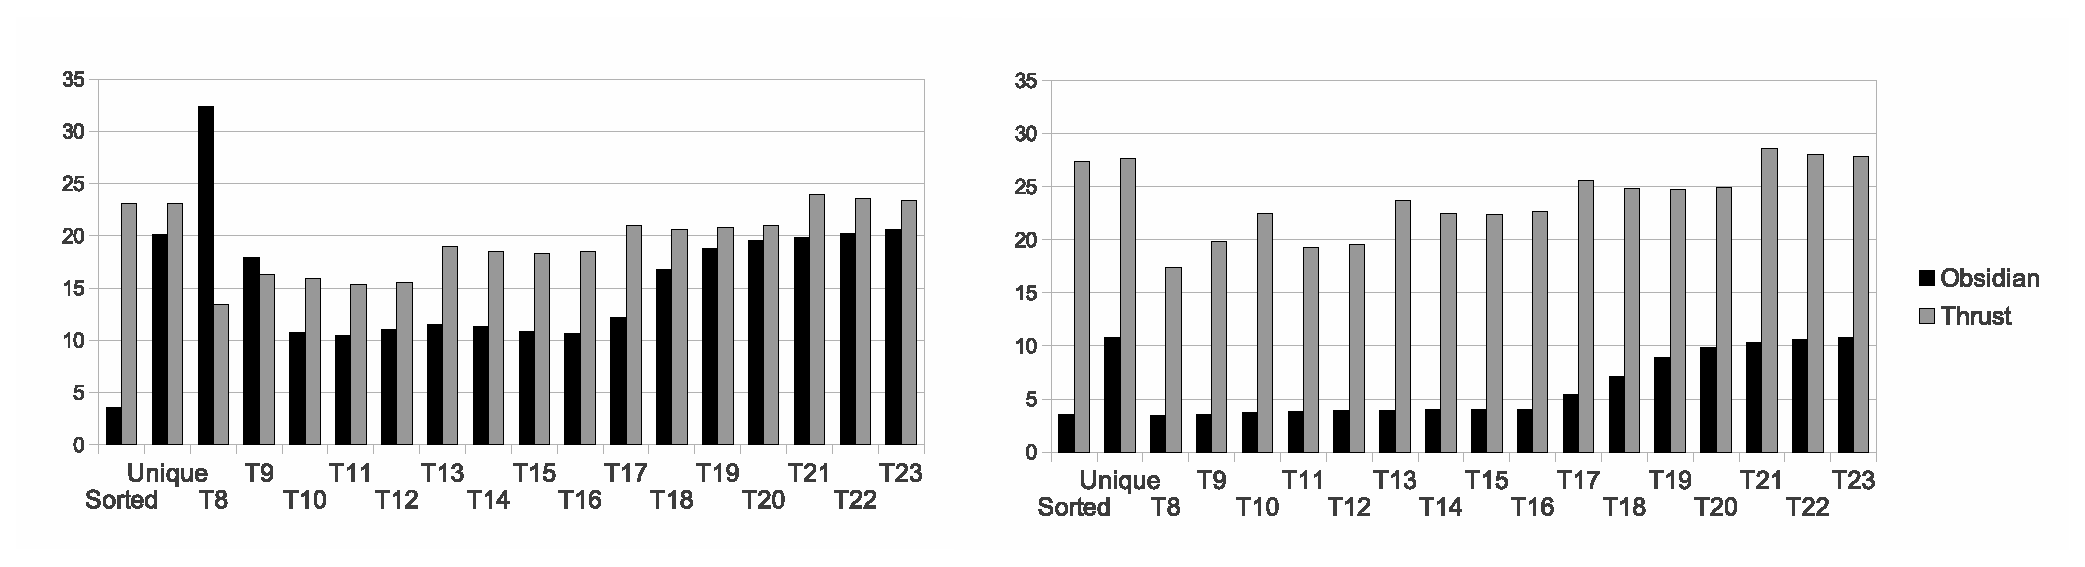
\includegraphics[width=\linewidth]{./img/chart1}
%\caption{Running time and parallel speedup of matrix 
%         multiplication on matrices of different size using ArBB}
%\label{fig:arbbchart}
%\end{figure}


%\begin{figure}
%\includegraphics[width=\linewidth]{./img/arbb1}
%\caption{Execution time for matrix-matrix multiplication using ArBB (C++).
%         Chart shows execution time for various sizes of matrices using 
%         either one two or four cores.}
%\label{fig:arbbchart}
%\end{figure}


%\begin{figure}
%\includegraphics[width=\linewidth]{./img/embarbb1}
%\caption{Execution time for matrix-matrix multiplication using EmbArBB.
%         Chart shows execution time for various sizes of matrices using 
%         either one, two or four cores.}
%\label{fig:embchart}
%\end{figure}

%\begin{figure}
%\includegraphics[width=\linewidth]{./img/repa1}
%\caption{Execution time for matrix-matrix multiplication using Repa.
%         Chart shows execution time for various sizes of matrices using 
%         either one, two, four or eight threads.}
%\label{fig:repachart}
%\end{figure}






%\begin{figure}
%\includegraphics[width=\linewidth]{./img/compare2}
%\caption{CAPTION HERE}
%\label{fig:compare2chart}
%\end{figure}




\FloatBarrier


%
\subsection {Discussion}

%% ** TODO. Mention CSE. warp-related opt.

Push arrays form a new approach to array representation in DSELs.
We do not know of similar approaches in the literature, despite
the fact that the notions of demand and data flow
may feel familiar to the reader who considers Pull and Push arrays.
The addition of Push arrays to Obsidian seems highly beneficial. With 
this new feature, the user gains finer grained control over the code generated
and the resulting CUDA kernels perform considerably better than before.
This 
was illustrated in the series of sorters explored in section~\ref{sec:MARY}.
The performance of {\tt vsort} is sufficiently good that it
can be used as a first phase in a larger sorter (written in CUDA) that
can sort 16M elements in 96 ms, while an i7-920 CPU takes
around 2740 ms. Further speed improvements look possible, both in the coordination code
and in the kernels. An obvious next step would be to investigate the generation of the {\tt iSwap} and
{\tt vSwap} kernels from Obsidian. (This is not currently possible because of assumptions that we made about the interfaces to kernels and about how {\em thread ids} are used. We will look into ways to relax
our assumptions.)

The series of kernels also illustrates how the use of combinators brings a form of reuse, and makes design exploration easier. Our experience of using similar combinators in the Lava hardware
description language~\cite{LavaSorter} was that a relatively small set of combinators went a long way. So, although we introduced three
combinators here, {\tt ilv}, {\tt vee} and {\tt ilvVee}, which
includes the other two, we do not believe that every new kernel development exercise would demand a completely new set of combinators.
We expect to provide the user with a well-documented set of combinators,
so that users can get access to this style of programming without having
to develop their own combinators, and without having to think too much
about bit-hacking.
The bit-manipulation approach chosen to define our combinators automatically
created functions that apply to sub-sequences of the input that
are of an appropriate length.

In this paper, we made combinators for the special case of two input, two
output operations (built from two two-input funtions that we typically called
{\tt f} and {\tt g}). 
This approach should be generalised to deal with blocks that have $2^k$ inputs
and outputs.
Also, we made a compound combinator from {\tt ilv} and {\tt vee},
but generalising to more than two input components would allow
for composing combinators, and indeed for recursive descriptions
that could be unrolled. Then, ignoring {\tt syncs}, a recursive description of
{\tt vsort} could be something like 
\begin{codesize}
\begin{verbatim}
vsortR 0 = id
vsortR n = bpmergeR n . ilv2 1 (vsortR (n-1))
\end{verbatim}
\end{codesize}
\noindent
It would then be necessary to optimise the code generated from
multiple applications of {\tt ilv2 1}, for example, whereas here
we have forced the user to figure out both the unrolling and the combinations.
Moving to more general combinators would also give the opportunity to
provide predefined combinators that capture more of the commonly used threading patterns (for instance $k$ indices per thread rather than the $1$ and $2$ shown here).

The integration of Push arrays into Obsidian raises some new questions.
Previously, there was a direct correspondence between the length 
of an array and the number of threads used to compute it, which
allowed the user to write an initial program without worrying about
threads at all, and then to tweak the Obsidian program if he was not satisfied
with the threading behaviour of the resulting kernel. 
Now, as can be seen in the {\tt catArrayPs} example and in the sorters, this correspondence
can be broken using Push arrays. The {\tt catArrayPs} example and two
of the sorters use half as many threads as the 
number of elements. For users who are very concerned about the speed of
the generated kernels, getting this control through using Push arrays in
a particular pattern is clearly a good thing. But adding a second, different
way to control thread use in the generated code certainly complicates matters, and further case studies are needed to confirm that the complication pays off.

The addition of Push arrays also adds the possibility to include potentially 
unsafe operations in Obsidian, for example by writing multiple array elements to the same index, or by discarding elements.
This new expressiveness will have to be carefully controlled. On the positive side, it offers the possibility to encode functions like {\tt filter} from Haskell
that
are simply not expressible using only Pull arrays. Being able to implement {\tt filter} would make programming kernels in obsidian feel much more like programming in Haskell -- a welcome loosening of the strait-jacket.
Once that is done, it will be time to develop a very simple coordination language to allow programming of entire GPU applications that make use of
the kind of small kernel building blocks developed here.






\subsection{Future Work} 
\label{sec:FutureWork}


%The Haskell - EmbArBB interface needs to be improved. 
%Currently there is a 
%transfer of data into ArBB before a function is executed and the results 
%are directly transferred back into Haskell.
%This is not ideal when several ArBB functions are composed, as this
%will lead to unnecessary copying of data into and out of ArBB.
%One possible solution would be to have the {\tt ArBB} monad keep track of what arrays have been bound 
%to ArBB variables and stored into ArBB memory.
%Another problem with the interface is the way {\tt map} works. Currently 
%{\tt map} takes an identifier pointing out a captured function. These
%captured functions are maintained by the {\tt ArBB} monad, which means that 
%either a function that maps some other function over data needs to be defined 
%in the {\tt ArBB} monad, or it needs to be passed the function as an argument 
%at capture time. Neither of those alternatives is desirable and new solutions
%will have to be found.



%One thought is to 
%also let the {\tt ArBB} monad keep track of what arrays have been bound 
%to ArBB variables and stored into ArBB memory. Currently there is a 
%transfer of data into ArBB before a function is executed and the results 
%are directly transferred back into Haskell. This is limiting in case 
%the programmer wants to execute several ArBB functions in sequence, each 
%on the result of the previous function. In this scenario data will be 
%copied back and forwards needlessly between function executions in the current 
%implementation. 


The C++ embedding of ArBB allows for dense containers of structs in some cases. 
The operations on vectors supplied by the ArBB virtual machine are exclusively 
over vectors of scalar types. So the C++ embedding must be performing a AOS to SOA 
(Array of Struct to Struct of Array) transformation. The Haskell embedding 
does not implement any similar transformation. This is an important addition 
that would for example make implementing functions on complex numbers easier. 

We stress that this paper presents first steps in the implementation of 
EmbArBB. Our benchmarks, while promising, are very limited. We must devote 
effort to developing a suite of interesting, larger data parallel programs 
for use in benchmarking EmbArBB. It is particularly important to explore the 
nested vectors, and the effects of the limitation to one level of nesting 
in ArBB. Those parts of ArBB that support nested vectors seem to be less well 
developed than those supporting dense vectors, as evidenced by the sample 
applications distributed with ArBB, none of which uses nesting. We expect 
ArBB to become more complete, and perhaps we will be able to contribute 
interesting examples both in the C++ and Haskell embeddings.

Having exercised EmbArBB more thoroughly, we will assess the results of 
the benchmarking and experiments with programming idioms, and decide on future
research directions. We expect to focus on ways to provide users with an interface that is more 
functional in style than the current C++ oriented one. 
%ArBB has nested vectors that are used to implement nested data parallelism, that 
%is data parallelism with irregularly shaped data, in the style of
%NESL~\cite{NESL}. The Haskell embedding has so 
%far been focused entirely on the dense functionality of ArBB. 
%The next step will be to find ways to embed the nested operations too.
%Looking on the 
%nested operations and seeing how these can be embedded as well is next in line. 


%GPUs are efficient on flat data parallel workloads, and approaches
%to GPU programming often offer only flat data parallelism.
%Although there is some promising recent work on nested data parallelism
%in a functional setting
%on GPUs~\cite{NestedGPU}, this area is generally less well explored.
%We are enticed by the idea of
%using EmbArBB as a 
%platform for exploration of GPU programming and nested data-parallelism.
%Implementing a GPU backend to EmbArBB would require applying 
%GPU specific optimisations to the EmbArBB AST (expression datatype). 
%The question of whether to perform the necessary optimisations
%at the EmbArBB level, or later, inside ArBB, is an interesting
%one that we would like to explore.



%However 
%if implementing a GPU backend on the EmbArBB level is the right thing to do 
%or if rather it should be implemented as part of the ArBB system? There 
%could be a point to explore in the setting of EmbArBB the space of different 
%optimisations and transformations needed to run the functions on a GPU before 
%doing it in the more complicated (perhaps) setting of full ArBB.  
  


\subsection{Conclusion} \label{sec:conc}

Obsidian provides a good interface for experimenting with algorithms on GPUs. 
The earlier version described in~\cite{JMT} showed that it is possible to 
generate efficient CUDA code from the kind of high level descriptions we are 
interested in. For the kernel level, the work in progress described in this paper enhances the  expressive power of Obsidian, extending the range of algorithms that can be described, as well as the degree of control exercised by the user. 
Future work will concentrate on improving the performance of the resulting 
applications, as well as on support for the kernel coordination level.
 

%\citeemb{joelryan}
%\citeemb{arbbpb}
%\citeemb{arbbcpp}
%\citeemb{arbbvm}
%\citeemb{ARBB2011}
%\citeemb{REPA}
%\appendix
%\section{Appendix Title}

%This is the text of the appendix, if you need one.

%\acks
\subsection*{Acknowledgments}
%** Note. Joel should thank Intel. We should ack funding from VR and SSF.
Svensson was first introduced to ArBB while on a three month internship at Intel
during 2011. Thanks go to Ryan R. Newton for inspiring supervision 
during that internship.
%while 
%working on Haskell bindings to ArBB at Intel as well as trying to understand 
%the intricate details of the inside of Data.Array.Accelerate. 

This research has been funded by the Swedish Foundation for
Strategic Research (which funds the Resource Aware Functional 
Programming (RAW FP) Project) and by the
Swedish Research Council.



% We recommend abbrvnat bibliography style.

\bibliographystyleemb{alpha}
\bibliographyemb{thesis}
\addcontentsline{toc}{subsection}{Bibliography}
% The bibliography should be embedded for final submission.

%% \begin{thebibliography}{}
%% \softraggedright
%% \bibitem[Axelsson et~al.(2010)Axelsson, Claessen, D{\'e}vai, Horv{\'a}th,
%%   Keijzer, Lyckeg{\aa}rd, Persson, Sheeran, Svenningsson, and
%%   Vajda]{FELDSPAR2010}
%% E.~Axelsson, K.~Claessen, G.~D{\'e}vai, Z.~Horv{\'a}th, K.~Keijzer,
%%   B.~Lyckeg{\aa}rd, A.~Persson, M.~Sheeran, J.~Svenningsson, and A.~Vajda.
%% \newblock Feldspar: {A} domain specific language for digital signal processing
%%   algorithms.
%% \newblock In \emph{8th ACM/IEEE International Conference on Formal Methods and
%%   Models for Codesign (MEMOCODE 2010)}, pages 169--178. IEEE Computer Society,
%%   2010.

%% \bibitem[Blelloch(1996)]{NESL}
%% G.~Blelloch.
%% \newblock Programming {P}arallel {A}lgorithms.
%% \newblock \emph{Communications of the ACM}, 39\penalty0 (3), 1996.

%% \bibitem[Chakravarty et~al.(2011)Chakravarty, Keller, Lee, McDonell, and
%%   Grover]{accelerate}
%% M.~M. Chakravarty, G.~Keller, S.~Lee, T.~L. McDonell, and V.~Grover.
%% \newblock {A}ccelerating {H}askell {A}rray {C}odes with {M}ulticore {GPU}s.
%% \newblock In \emph{Proceedings of the sixth workshop on Declarative aspects of
%%   multicore programming}, DAMP '11, pages 3--14, New York, NY, USA, 2011. ACM.
%% \newblock ISBN 978-1-4503-0486-3.
%% %\newblock \doi{10.1145/1926354.1926358}.
%% \newblock URL \url{http://doi.acm.org/10.1145/1926354.1926358}.

%% \bibitem[Elliott et~al.(2003)Elliott, Finne, and de~Moor]{ELLIJFP}
%% C.~Elliott, S.~Finne, and O.~de~Moor.
%% \newblock Compiling embedded languages.
%% \newblock \emph{Journal of Functional Programming}, 13\penalty0 (2), 2003.
%% \newblock URL \url{http://conal.net/papers/jfp-saig/}.

%% \bibitem[Gill(2009)]{Gill}
%% A.~Gill.
%% \newblock Type-{S}afe {O}bservable {S}haring in {H}askell.
%% \newblock In \emph{Proceedings of the 2009 ACM SIGPLAN Haskell Symposium},
%%   09/2009 2009.
%% \newblock URL
%%   \url{http://www.ittc.ku.edu/csdl/fpg/sites/default/files/Gill-09-TypeSafeRei%
%% fication.pdf}.

%% \bibitem[Hughes and Sheeran(2012)]{TFPIEPFP}
%% J.~Hughes and M.~Sheeran.
%% \newblock Teaching parallel functional programming at {C}halmers.
%% \newblock In \emph{presentation at Trends in Functional Programming in
%%   Education, Workshop associated with Conf. on Trends in Functional
%%   Programming, St. Andrews}, 2012.

%% \bibitem[Intel()]{arbbvm}
%% Intel.
%% \newblock {I}ntel(r) {A}rray {B}uilding {B}locks {V}irtual {M}achine
%%   {S}pecification.
%% \newblock \url{http://software.intel.com/sites/whatif/arbb/arbb_vm.pdf}.

%% \bibitem[Keller et~al.(2010)Keller, Chakravarty, Leshchinskiy, Peyton~Jones,
%%   and Lippmeier]{REPA}
%% G.~Keller, M.~M. Chakravarty, R.~Leshchinskiy, S.~Peyton~Jones, and
%%   B.~Lippmeier.
%% \newblock Regular, shape-polymorphic, parallel arrays in haskell.
%% \newblock In \emph{Proceedings of the 15th ACM SIGPLAN international conference
%%   on Functional programming}, ICFP '10, pages 261--272, New York, NY, USA,
%%   2010. ACM.
%% \newblock ISBN 978-1-60558-794-3.
%% %\newblock \doi{10.1145/1863543.1863582}.
%% \newblock URL \url{http://doi.acm.org/10.1145/1863543.1863582}.

%% \bibitem[Lippmeier et~al.(2012)Lippmeier, Chakravarty, Keller, Leshchinskiy,
%%   and Jones]{DPH}
%% B.~Lippmeier, M.~M.~T. Chakravarty, G.~Keller, R.~Leshchinskiy, and S.~P.
%%   Jones.
%% \newblock {W}ork {E}fficient {H}igher-{O}rder {V}ectorisation.
%% \newblock \url{http://www.cse.unsw.edu.au/~chak/papers/replicate-tr.pdf}, 2012.
%% \newblock ICFP'12.

%% \bibitem[Mainland and {M}orrisett(2010)]{NIKOLA}
%% G.~Mainland and G.~{M}orrisett.
%% \newblock Nikola: {E}mbedding {C}ompiled {GPU} {F}unctions in {H}askell.
%% \newblock In \emph{Proceedings of the third ACM Haskell symposium}, pages
%%   67--78. ACM, 2010.
%% \newblock ISBN 978-1-4503-0252-4.
%% \newblock URL \url{http://doi.acm.org/10.1145/1863523.1863533}.

%% \bibitem[Newburn et~al.(2011)Newburn, So, Liu, McCool, Ghuloum, Toit, Wang, Du,
%%   Chen, Wu, Guo, Liu, and Zhang]{ARBB2011}
%% C.~J. Newburn, B.~So, Z.~Liu, M.~McCool, A.~Ghuloum, S.~D. Toit, Z.~G. Wang,
%%   Z.~H. Du, Y.~Chen, G.~Wu, P.~Guo, Z.~Liu, and D.~Zhang.
%% \newblock Intel's array building blocks: A retargetable, dynamic compiler and
%%   embedded language.
%% \newblock In \emph{Proceedings of the 2011 9th Annual IEEE/ACM International
%%   Symposium on Code Generation and Optimization}, CGO '11, pages 224--235,
%%   Washington, DC, USA, 2011. IEEE Computer Society.
%% \newblock ISBN 978-1-61284-356-8.

%% \bibitem[Sheeran(2004)]{LavaMultipliers}
%% M.~Sheeran.
%% \newblock Generating fast multipliers using clever circuits.
%% \newblock In \emph{Int. Conf. on Formal Methods in Computer Aided Design
%%   (FMCAD)}, volume 3312 of \emph{LNCS}, pages 6--20, 2004.

%% \bibitem[Sheeran(2011)]{SheeranJFP}
%% M.~Sheeran.
%% \newblock Functional and dynamic programming in the design of parallel prefix
%%   networks.
%% \newblock \emph{J. Funct. Program.}, 21\penalty0 (1):\penalty0 59--114, 2011.

%% \bibitem[Svensson and Newton(2011)]{joelryan}
%% B.~J. Svensson and R.~Newton.
%% \newblock {P}rogramming {F}uture {P}arallel {A}rchitectures with {H}askell and
%%   {A}r{BB}.
%% \newblock \url{http://faspp.ac.upc.edu/faspp11/pdf/faspp11-final12.pdf}, 2011.
%% \newblock Presented at the workshop: {F}uture {A}rchitectural {S}upport for
%%   {P}arallel {P}rogramming (FASPP), in conjuction with ISCA '11.


%% \end{thebibliography}
%% %\bibliography{paper}

%% \end{document}
